\documentclass[12pt]{article}
 
\usepackage[table]{xcolor}
\usepackage[margin=1in]{geometry} 
\usepackage{amsmath,amsthm,amssymb,wasysym}
\usepackage{pgf,tikz,pgfplots}
\usepackage{mathrsfs}
\usepackage{mathtools}
\usepackage{listings}
\usepackage{colortbl}
\usepackage{verbatim}
\usetikzlibrary{arrows, angles, quotes, decorations.pathreplacing, math, patterns}
\usepackage{framed}
\usepackage{graphicx}
\graphicspath{ {./images/} }

\lstset{basicstyle=\footnotesize}
\usetikzlibrary{calc}

\newcommand{\N}{\mathbb{N}}
\newcommand{\Z}{\mathbb{Z}}
\newcommand{\I}{\mathbb{I}}
\newcommand{\R}{\mathbb{R}}
\newcommand{\Q}{\mathbb{Q}}
\DeclarePairedDelimiter{\ceil}{\lceil}{\rceil}
 
\begin{document}
 
\title{Induction\\
    \large CS101A Problem Solving I}
\author{Harry Coleman}
\date{November 12, 2019}

\maketitle

\section*{Problem 1}
\fbox{
    \parbox{\textwidth} {
        Prove that $|\sin{nx}| \leq n|\sin{x}|$ for any real number $x$ and positive integer $n$.
    }
}
\\

To show this inductively, we'll let $x$ be any real number. we consider $n=1$ as our base case
\begin{align*}
    |\sin{nx}| &\leq n|\sin{x}| \\
    |\sin{x}| &\leq |\sin{x}|
\end{align*}
and this is clearly true. For the inductive step, we assume that for some positive integer $n$,
\[|\sin{nx}| \leq n|\sin{x}|\]
and we want to show
\[|\sin{((n+1)x)}| \leq (n+1)|\sin{x}|\]

Consider
\[|\sin{((n+1)x)}| = |\sin{(nx + x)}|\]
Using the sum of angles trig identity, we get this to be
\[=|\sin{nx}\cos{x} + \cos{nx}\sin{x}|\]
and with some absolute value properties, we get this to be
\[\leq|\sin{nx}||\cos{x}| + |\cos{nx}||\sin{x}|\]
Since $0\leq \cos{x}\leq 1$, this is
\[\leq|\sin{nx}| + |\sin{x}|\]
and by our inductive hypothesis,
\[\leq n|\sin{x}|+|\sin{x}|\]
\[=(n+1)|\sin{x}|\]
so
\[|\sin{((n+1)x)}| \leq (n+1)|\sin{x}|\]

So by the principle of induction, for any $x\in\R$ and $n\in\Z^+$, $|\sin{nx}| \leq n|\sin{x}|$.

\newpage
\section*{Problem 3}
\fbox{
    \parbox{\textwidth} {
        The plane is divided into regions by straight lines. Show that it is always possible to color the region with two colors so that adjacent regions are never the same color (like a checkerboard).
    }
}
\\

We will show inductively that this is true for all planes separated by $n\in\N$ lines. The base case would be zero lines, in which the whole plane is one region, which could be colored any one color to satisfy the property.

For the inductive step, we will show that if a plane separated by $k\in\N$, for all $0\leq k\leq n$ where $n\in\N$, lines can be checker-colored, then a plane separated by $n+1$ lines can be checker-colored.

First, we will assume that we have some valid region separated by $n$ lines. For example:
\begin{center}
    
\includegraphics[scale=0.09]{amthgoodcjeckers.png}    
\end{center}

If we add in a new line to the plane, we obtain two regions on either side of the new line. Each of these regions will have some number of lines less than or equal to $n$. If there are any lines parallel to the new line, then for each parallel line on one side of the new line, the other side has one less line. This means each side, on it's own, satisfies the checkering property.
\begin{center}
    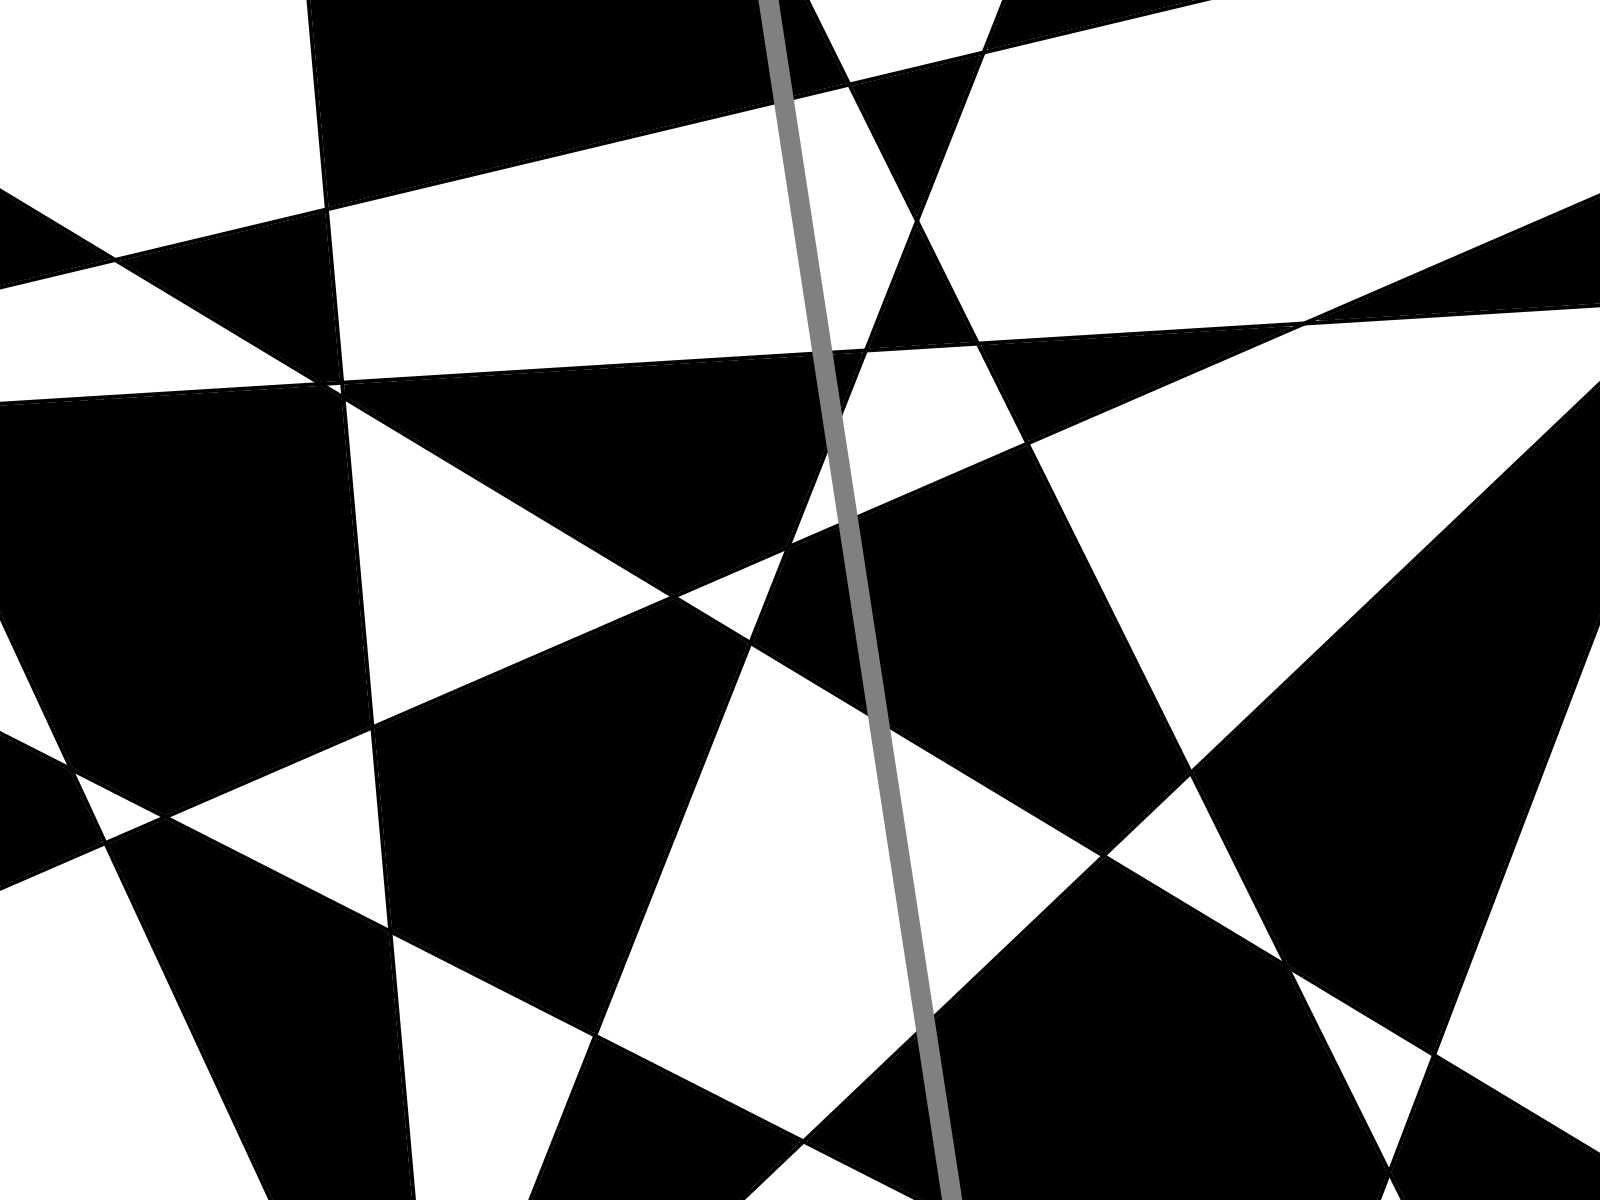
\includegraphics[scale=.09]{line.png}
\end{center}

The only adjacent regions of the same color are those separated by our new line. Not only that, but every pair of regions adjacent at the new line are the same color, since this new line separated existing regions and no colors changed.

If we now invert all the coloring on one side of the new line, we will still have each side independently satisfy the checkering property. We will also no longer have any adjacent regions of the same color at the new line, since for every pair of adjacent regions at the new line, both were the same color, then one had its color inverted.
\begin{center}
    
\includegraphics[scale=.09]{flipped.png}
\end{center}

Therefore, we have a valid checkering for a plane with $n+1$ lines. By the principle of strong induction, a plane separated by any $n\in\N$ lines can be checker-colored.

\section*{Problem 5}
\fbox{
    \parbox{\textwidth} {
        Let $P(n)$ be the statement: In any group of $n$ people, everyone in that group has the same age.
        \begin{itemize}
            \item In any group of one person, everyone in the group has the same age. That is $P(1)$ is true.
            \item Now we assume that $P(k)$ is true and look at a group of $k+1$ people which we call $G$. We want to show that everyone in the group $G$ is of the same age. To do that it is enough to show that any two members of the group $G$ have the same age. So let $Q$ and $S$ be arbitrary distinct members of the group $G$. Now consider everybody in $G$ except $S$, call this group of people $W$. $W$ is a group of $k$ people and since $P(k)$ is true, everyone in $W$ is of the same age. Next consider everybody in $G$ except $Q$; call this group of people $R$. $R$ is a group of $k$ people and since $P(k)$ is true, everyone in $R$ is of the same age. Now pick an individual $X$ that is in both $W$ and $R$. Then, since $X$ and $Q$ are both members of $W$, they are of the same age. Likewise, $X$ and $S$ are both members of $R$ and are therefore the same age. Thus $Q$ and $S$ are of the same age.
        \end{itemize}
        Now we have proved the statement $P(n)$ for every natural number $n$. The statement is certainly not true so there is something wrong in the proof. Where is the error?
    }
}
\\

Because the inductive step defines
\[W = G \setminus\{S\}\]
\[R = G \setminus\{Q\}\]
and supposes the existence of $X$ which is an element of $W$ and $R$, $G$ must have at least 3 distinct elements $Q,S,R$. However, if we consider the case of $k=1$, then $G$ would have $k+1=2$ elements, so supposing the existence of $X$ leads to the contradiction that $G$ must have at least 3 elements. So the inductive step is invalid.


\newpage
\section*{Problem 6}
\fbox{
    \parbox{\textwidth} {
        The sequence $a_0,a_1,a_2,\dots$ satisfies
        \[a_{m+n}+a_{m-n} = \frac{1}{2}(a_{2m}+a_{2m})\]
        for all nonegative integers $m$ and $n$ with $m\geq n$. if $a_1=1$ determine $a_{2009}$.
    }
}
\\

We claim that the sequence $a_0,a_1,a_2,\dots$ such that
\[a_i = i^2\]
satisfies this property. With this, we can simplify the given equation
\[a_{m+n}+a_{m-n} = \frac{1}{2}(a_{2m}+a_{2m})\]
by substituting for all $a_i$ terms with $i^2$. So
\begin{align*}
    (m+n)^2+(m-n)^2 &= \frac{1}{2}((2m)^2+(2m)^2) \\
    m^2 + 2mn + n^2 + m^2 - 2mn + n^2 &= \frac{1}{2}(4m^2+4n^2) \\
    2m^2 + 2n^2 &= 2m^2 + 2n^2 \\
    0 &= 0 \\
\end{align*}

Since this is a tautology, it is clear that our assignment of $a_i=i^2$ will satisfy $0=0$ for all $i\in\N$. So
\[a_{2009} = 2009^2 = 403608\]

\newpage
\section*{Problem 8}
\fbox{
    \parbox{\textwidth} {
        Show that every positive integer can be written as a sum of distinct terms of the Fibonacci sequence.
    }
}
\\

For terms of the Fibonacci sequence, we have that
\[t_i + t_{i+1} = t_{i+2}\]
or
\begin{equation}
    t_{i-1} + t_i = t_{i+1} \label{diff}
\end{equation}
and that
\begin{equation}
    t_i < t_{i+1} \label{ineq}
\end{equation}

We want to show that for all $n\in\N$, we can write $n$ as a sum of distinct terms of the Fibonacci Sequence. Our base case is simple, since the smallest positive integer, 1, can be written as the Fibonacci term, 1.

For the inductive step, we'll assume that for some $n\in\N$, we have that for all $k\in\N$ such that $k\leq n$, $k$ can be written as a sum of distinct terms of the Fibonacci sequence. We now want to show that $n+1$ can be written as a sum of distinct terms of the Fibonacci sequence.

Consider the greatest Fibonacci term less than or equal to $n+1$, call this $t_r$. So we can say
\[n+1 = t_r + a\]
where $a=(n+1)-t_r$ and $a\in\N$ or $a=0$. If $a=0$, then $n+1$ is the Fibonacci term $t_r$. Otherwise, $a < n+1$, so $a\leq n$. So by our inductive hypothesis, $a$ can be written as the sum of distinct terms of the Fibonacci Sequence. And since
\[n+1 = t_r + a\]
$n+1$ can be written as a sum of Fibonacci terms. However, to show that the terms are distinct, we must show that $t_r$ is not one of the terms in the sum for $a$. By our definition of $t_r$ as the greatest term less than or equal to $n+1$, we have
\begin{align*}
    n+1 &< t_{r+1} \\
    (n+1) - t_r &< t_{r+1} - t_r \\
    a &< t_{r-1} \quad \text{by \eqref{diff}}\\
    a &< t_r \qquad\text{by \eqref{ineq}}
\end{align*}

So $t_r$ is not in the sum of distinct Fibonacci terms for $a$. So we can have $n+1 = t_r +$(the distinct Fibonacci terms which sum to a), where all the terms are distinct. So $n+1$ can be written as the sum of distinct terms of the Fibonacci Sequence. So by the principle of strong induction, we have that for all $n\in\N$, $n$ can be written as a sum of distinct terms of the Fibonacci Sequence.


\end{document}